E' richiesto un set di immagini con le seguenti specifiche: 
\begin{itemize}
    \item 8 Immagini di dimensione $512 \times 512$;
    \item Formato PNG in scala di grigi;
    \item Devono contenere tra i 2 ed i 6 oggetti geometrici;
    \item Oggetti di colore uniforme su uno sfondo nero.
\end{itemize}
\begin{figure}[h]
    \centering
    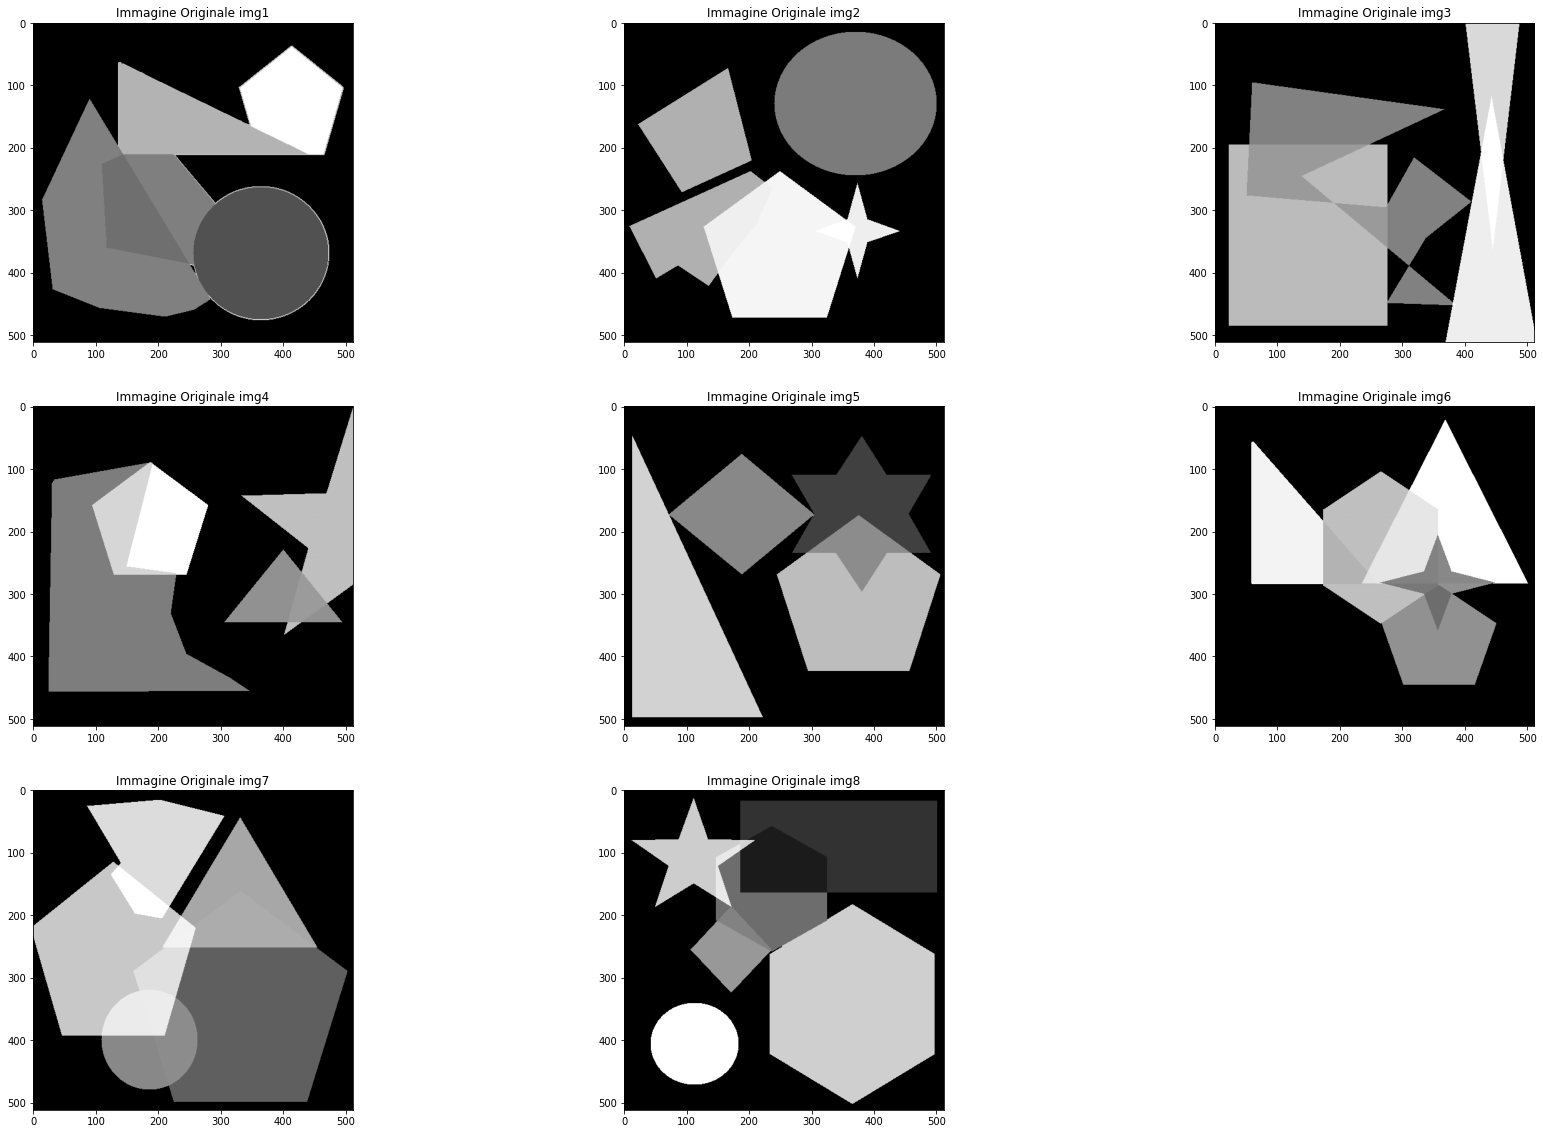
\includegraphics[width=0.5\linewidth]{./imgRel/dataset.png}\label{fig:datasetgeometriche}
    \caption{Immagini geometriche utilizzate}
\end{figure}
Useremo anche altre due immagini di tipo fotografico/medico/astronomico a scelta trovate su internet.
Quest'ultime saranno importate all'interno del progetto con la libreria \code{skimage}, impostando il flag \verb|as_gray=True| per averle in bianco e nero.

Le immagini selezionate sono le seguenti:
\begin{description}
    \item[Immagine Fotografica] Mostra un fotografo nell'intento di uno scatto con sfondo paesaggistico.
    \item[Immagine Ritratto] Ritrae il volto di una persona in modo dettagliato e con varie tonalità di grigio.
\end{description}

\begin{figure}[h]
    \centering
    \begin{subfigure}{0.5\textwidth}
        \centering
        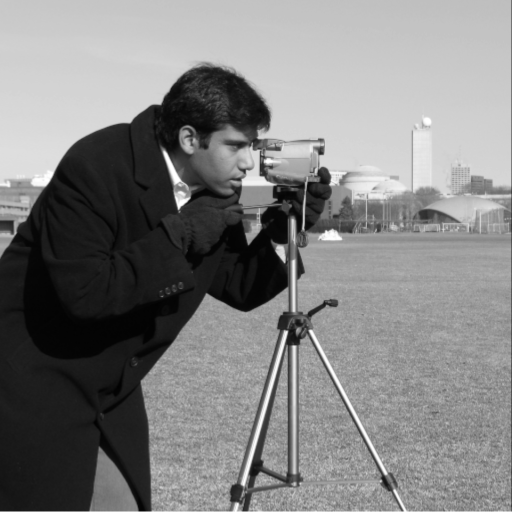
\includegraphics[width=0.5\linewidth]{./img/datacamera.png}\label{fig:giornale}
        \subcaption{Immagine fotografica}
    \end{subfigure}\hfill
    \begin{subfigure}{0.5\textwidth}
        \centering
        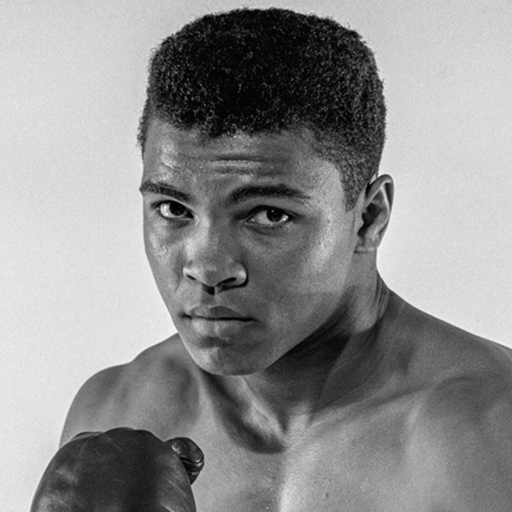
\includegraphics[width=0.5\linewidth]{./img/pugile.png}\label{fig:pugile}
        \subcaption{Immagine ritratto}
    \end{subfigure}
    
    \caption{Immagini fotografiche analizzate}
\end{figure}
